The Genius Invocation TCG is a card game that has taken Teyvat by storm. In this game, each character card boasts three unique skills. At the outset of every turn, players acquire a set number of dice through rolls. Each die can represent one of seven elements or be a colorless die, and players can expend these dice to unleash a variety of skills.

The Cat's Tail in Mondstadt frequently hosts showdowns in the heated battle mode of the Genius Invocation TCG. This mode often features a plethora of unconventional rules, such as reducing the number of dice needed for skills or making all dice colorless.

Now, let's delve into a simplified version of the heated battle mode where all dice are colorless. Normal attacks and elemental skills require only $1$ die, while elemental bursts demand $2$ dice, and no charging is necessary. In this scenario, only one character occupies the battlefield.

To optimize resource utilization, the goal is to determine the number of ways to exhaust all the dice.

To be specific, starting with $k$ dice, you can execute the following three operations until you have $0$ dice remaining:

\begin{itemize}
\item Normal attack, consuming $1$ die.
\item Elemental skill, consuming $1$ die.
\item Elemental burst, consuming $2$ dice.
\end{itemize}

Two sequences of operations are considered distinct if and only if their total numbers of operations differ or if there exists an $i$ such that the $i$-th operation in the two sequences differs.

As the result could be extremely large, you only need to output the result modulo $998244353$.


\begin{center}
  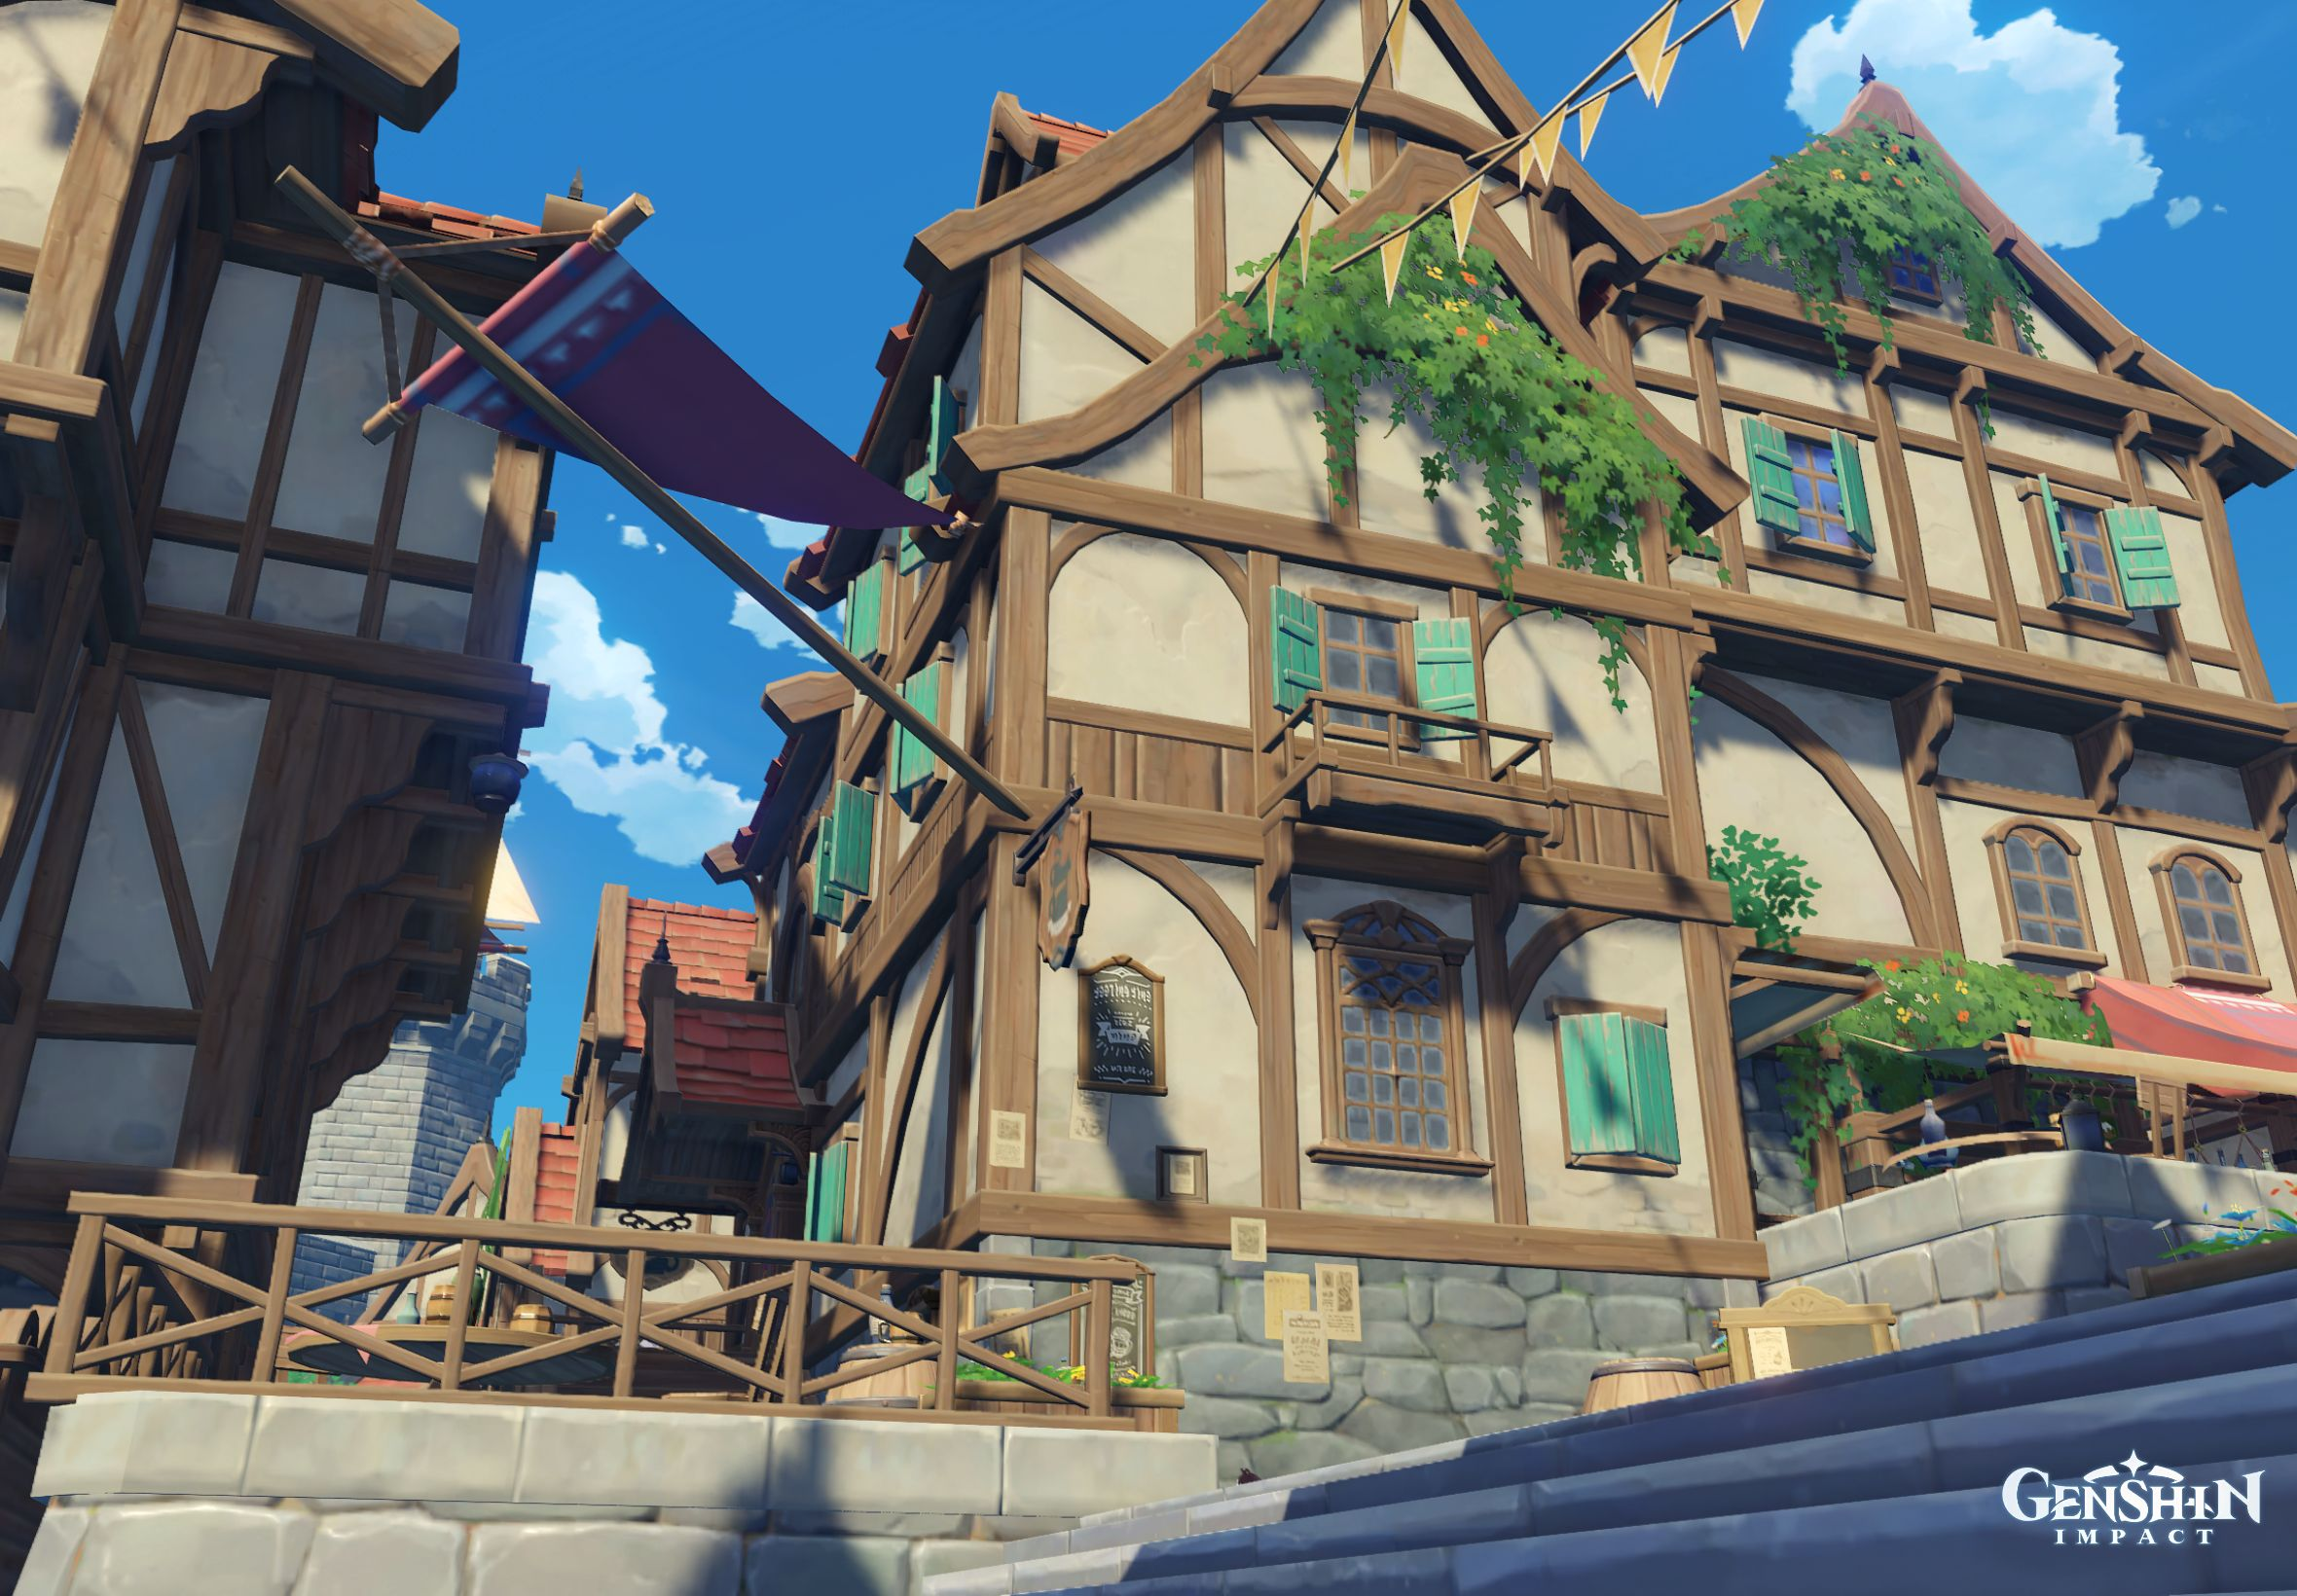
\includegraphics[scale=0.15]{cattail.jpg} \\
  \small{The Cat's Tail}
\end{center}
